\section{Pandosia}\label{pandosia}

Tags: Città Creatore: Lorenzo Ispirazione: Mendicino

\section{Pandosia}\label{pandosia-1}

\begin{center}\rule{0.5\linewidth}{0.5pt}\end{center}

Informazioni Generali

\begin{figure}
\centering
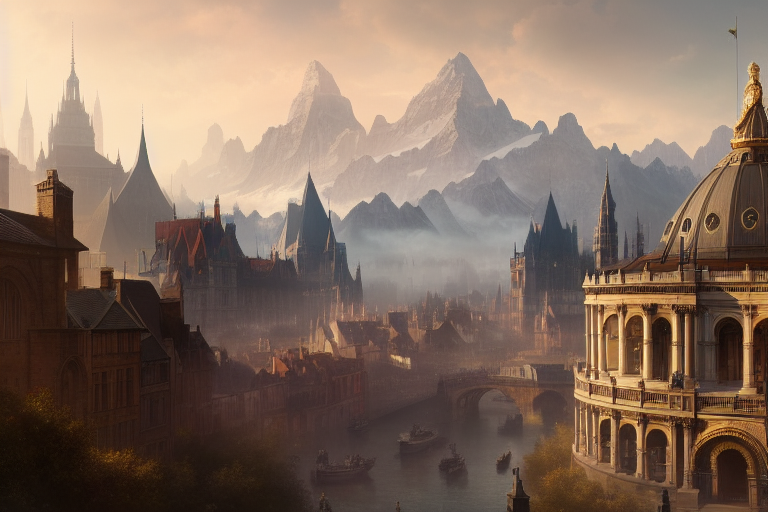
\includegraphics{draw-a-city-and-a-montain-haze-ultra-detailed-film-photography-light-leaks-larry-bud-melman-tr.png}
\caption{draw-a-city-and-a-montain-haze-ultra-detailed-film-photography-light-leaks-larry-bud-melman-tr.png}
\end{figure}

Tipo di Luogo: Città Minore

Dimensioni:

Altitudine: 650 m slm

Popolazione: 17000

Paese:

Luogo: Valtara

\begin{center}\rule{0.5\linewidth}{0.5pt}\end{center}

\subsection{1. Descrizione Generale}\label{descrizione-generale}

\begin{center}\rule{0.5\linewidth}{0.5pt}\end{center}

Pur non essendo particolarmente grande, riveste un ruolo importante come
centro produttivo per la seta e altri tessuti. La sua posizione
strategica lungo il corso del fiume Busento e nelle vicinanze della
catena montuosa della Sila ne fa un punto di riferimento per il
commercio e l'artigianato. La città è conosciuta per la sua vivace
atmosfera e per la bellezza dei suoi paesaggi naturali.

\subsection{2. Storia}\label{storia}

\begin{center}\rule{0.5\linewidth}{0.5pt}\end{center}

Non si conosce molto sulla storia della città. Probabilmente è sempre
stato un centro abitato tranquillo e dedito al commercio, che di rado ha
dovuto fare i conti con i numerosi conflitti che hanno interessato la
regione. Nonostante questa fortunata condizione, alcuni storici
Pandosiani affermano che il noto condottiero Al Riko, che guidò le
armate dishartane durante il secolo delle razzie, venne fermato e
sconfitto proprio dai Pandosiani. Non solo non ci sono prove che possano
confermare questo evento, ma è stato anche ampiamente dimostrato che il
condottiero si spinse fino alla città di Kos, ben oltre i confini della
città.

\subsection{3. Geografia}\label{geografia}

\begin{center}\rule{0.5\linewidth}{0.5pt}\end{center}

Pandosia si estende lungo le sponde del fiume Busento, che fornisce una
fonte vitale di acqua e risorse per la città. La sua posizione a ridosso
della catena montuosa della Sila le conferisce una vista spettacolare
sulle maestose vette e offre opportunità per l'esplorazione e
l'avventura. I paesaggi circostanti sono caratterizzati da colline
lussureggianti, boschi rigogliosi e prati fertili, creando una cornice
naturale incantevole per la città.

\subsection{4. Cultura}\label{cultura}

\begin{center}\rule{0.5\linewidth}{0.5pt}\end{center}

Pandosia è una città con una ricca cultura, influenzata dalle diverse
razze che la compongono. La lavorazione della seta è una delle arti più
pregiate, e le botteghe artigiane sono abbondanti nelle strade, con
tessitori e sarti che creano capi di abbigliamento pregiati e ricercati.
La cucina è un'altra forma d'arte celebrata nella città, con ristoranti
e taverne che offrono piatti deliziosi preparati dagli abili chef
halfling. La città ospita anche una serie di festival e celebrazioni
annuali, inclusa la cerimonia dell'elezione del questore ogni cinque
anni, che attira visitatori da tutto il Nord-Ovest.

\subsection{5. Demografia}\label{demografia}

\begin{center}\rule{0.5\linewidth}{0.5pt}\end{center}

La popolazione di Pandosia è variegata, ma gli abitanti sono
principalmente composti da orchi (42\%) e halfling (12\%). Questa
miscela di razze crea una vibrante fusione di culture e tradizioni nella
città. Gli orchi, noti per la loro forza e abilità nella produzione di
tessuti, hanno portato avanti l'antica tradizione della lavorazione
della seta, mentre gli halfling hanno contribuito con la loro abilità
culinaria e la loro propensione al commercio.

\subsection{6. Governo}\label{governo}

\begin{center}\rule{0.5\linewidth}{0.5pt}\end{center}

Pandosia è governata da un questore, un individuo eletto ogni cinque
anni per amministrare la città e risolvere le dispute tra i cittadini.
Il questore rappresenta l'autorità centrale e ha il compito di garantire
l'ordine e la prosperità all'interno di Pandosia. Le decisioni
importanti vengono prese in base al consenso tra i cittadini e i leader
delle diverse razze presenti nella città, promuovendo così la
cooperazione e la convivenza pacifica tra le diverse comunità. Il
Questore di Pandosia è anche uno dei membri del Consiglio della Gilda
dei Commercianti del Nord-Ovest.
